%\documentclass[11pt, draft, oneside]{report}
\documentclass[11pt]{report}
%\makeindex
%\usepackage{german,a4,showidx} %index an seite
\usepackage{german,a4}
%for pdfLaTeX output Bilder als .png speichern:
%\usepackage[pdftex]{graphicx} \DeclareGraphicsExtensions{.png}  \graphicspath{{bilder/png/}}
% f\"{u}r normales LaTeX->dvi, Bilder als .eps speichern:
\usepackage{graphicx} \DeclareGraphicsExtensions{.eps} \graphicspath{{bilder/eps/}}

%Definition der Seitengr"osse
\setlength{\textwidth}{15 true cm}
\setlength{\textheight}{22 true cm}
\oddsidemargin  0.5 cm
\evensidemargin 0.5 cm
\topmargin      0 cm

\selectlanguage{german}
%Beispiel fuer ein neues LaTex Kommando
\newcommand{\QSIM}{{\sc QSim}}

\begin{document}

% Die Titelseite ist immer in Deutsch (austrian), danach h\"{a}ngt es von der
% Sprache der Diplomarbeit ab. Jedenfalls muss eine Kurzfassung und
% ein Abstract existieren

%\thispagestyle{empty} 
%\selectlanguage{german}

\newpage
\vspace*{2.2 cm}
{\Large
\noindent
{\bf Kurzfassung}} \\
\vspace*{0.3 cm}

\noindent
Hier steht der deutsche Text der Kurzfassung. Eine
evtl. gek\"{u}rzte Version inklusive einiger Stichw\"{o}rter muss auch im
TUG-Online eingegeben werden.


\newpage
\selectlanguage{english}
\vspace*{2.2 cm}
{\Large
\noindent
{\bf Abstract}} \\
\vspace*{0.3 cm}

\noindent
This is the English version of the abstract.  It is also
required to submit a short English abstract including some
keywords to the TUG-Online system.

\newpage
\selectlanguage{german}
\newpage
\vspace*{2.2 cm}
{\Large
\noindent
{\bf Danksagung}} \\
\vspace*{0.3 cm}
% OPTIONAL

\noindent
Diese Diplomarbeit wurde im (Studien)Jahr am Institut f\"{u}r
Technische Informatik an der Technischen Universit\"{a}t Graz
durchgef\"{u}hrt.

\smallskip
Danksagung an alle am Institut bzw. bei Firmen, die geholfen
haben....

\medskip
Danksagung an Freunde und Freundinnen f\"{u}r das Verst\"{a}ndnis, ebenso
den Eltern und allen sonstigen Sponsoren....

\vspace{2 cm}

\noindent Graz, im Monat Jahr \hfill Name des Diplomanden

\newpage
% Inhaltsverzeichnis
\tableofcontents  

% Tabellenverzeichnis
% OPTIONAL
\listoffigures 

% Abbildungsverzeichnis
% OPTIONAL
\listoftables

%Seitennummerierung am Kopf inkl. Kapitel"uberschrift
\pagestyle{headings}
\chapter{Einleitung}
% Einleitung ist Kapitel 1
\label{kap:Einleitung} 
Dieses Dokument soll als Vorlage zum Verfassen von Diplomarbeiten am
Institut f"ur Technische Informatik der TU Graz mit Hilfe von \LaTeX\
dienen.  Es sind hier die wichtigsten Abschnitte der Diplomarbeit 
zusammengefa\3t.  Weiters werden die wichtigsten Befehle von \LaTeX\ an
einigen Beispielen kurz vorgestellt.  Dieses Vorlage erhebt keinen Anspruch
auf Vollst"andigkeit.

Die Einleitung enth\"{a}lt u.A. die Aufgabenstellung, die Vorgehensweise zur
L\"{o}sung und die Gliederung der Arbeit.  Es folgt nun ein {\bf Beispieltext}.

\section{Motivation}

Qualitative Simulation ist ein Teilbereich des {\em qualitative reasonings} 
(qualitatives Schlie\3en). Dabei wird versucht, Schlu\3folgerungen "uber 
das Verhalten von Systemen auf h"oheren Abstraktionsebenen zu ziehen.
Hauptanwendungsgebiete f"ur die qualitative Simulation sind Bereiche der 
k"unstlichen Intelligenz. 
Die Abbildung~\ref{fig_abstraktion} zeigt die verschiedenen Abstraktionsebenen eines 
Systems.  Die erste Ebene stellt das physikalische System dar. 
Durch die Beobachtung des Systems kann das Verhalten bestimmt werden.
In der zweiten Ebene wird das physikalische System mit 
Differentialgleichungen {\em (DGLen)} modelliert.  Durch eine analytischen 
Berechnung der DGLen wird eine Beschreibung des Verhaltens mit 
reell\-wertigen Funktionen erzielt.  In der kontinuierlichen Simulation 
werden h"aufig numerische Verfahren zur Berechnung dieser Funktionen 
eingesetzt.  Eine weitere Abstraktion der DGLen in qualitative DGLen 
{\em (qualitative differential equations - QDEs)} wird in der dritten Ebene 
vollzogen.  Die qualitative Simulation bestimmt aus diesem Modell eine 
qualitative Beschreibung des Systemverhaltens. 

\begin{figure} %optinale Positionsparameter [htbp]
\centerline{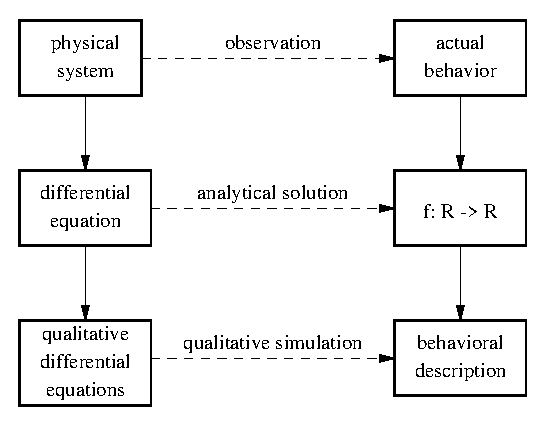
\includegraphics[width=10cm,keepaspectratio=true]{qdeode}}
%\centerline{\includegraphics[width=\the\columnwidth,keepaspectratio=true]{odeqde}}
\caption[Abstraktionsebenen eines physikalischen Sy\-stems.]
{Die verschiedenen Abstraktionsebenen eines physikalischen Sy\-stems.}
\label{fig_abstraktion}
\end{figure}

Im Gegensatz zur kontinuierlichen Simulation, welche f"ur numerische 
Eingabegr"o\3en die resultierenden Ausgabewerte berechnet, wird bei der 
qualitativen Simulation das Modell abstrakter betrachtet.
Diese abstrakte Betrachtungsweise entspricht auch eher dem menschlichen
Verst"andnis.
Gr"unde f"ur den Einsatz der qualitativen Simulation sind unter anderem:

\begin{itemize}
\item Das quantitative Wissen "uber ein System ist unvollst"andig oder 
nicht gegeben. 
\item Das Modell ist zu komplex und daher zu zeitaufwendig f"ur die 
konti\-nuier\-liche  Simulation.
\item Bestimmte Anwendungen ben"otigen gar nicht die detaillierten Ergebnisse der kontinuierlichen Simulation. Qualitative Aussagen sind ausreichend. 
\end{itemize}

Aufgrund dieser Eigenschaften wird die qualitative Simulation immer "ofter 
auch in technischen Anwendungen, wie zum Beispiel in der Proze\3- und 
Design"uberwachung oder in der Fehlerdiagnose, eingesetzt. \\

Der bekannteste Algorithmus f"ur die qualitative Simulation ist 
\QSIM~\cite{Kui94}..
Am Institut f"ur Technische Informatik wurde ein Forschungsprojekt 
gestartet, um die Laufzeit von \QSIM\ zu reduzieren. 
Im Rahmen dieses Projektes werden Coprozessoren f"ur rechenzeitintensive 
Teilfunktionen entwickelt und Parallelisierungm"oglichkeiten untersucht.


\section{Zielsetzung}

In dieser Arbeit wird die parallele Implementierung von rechenzeitintensiven 
Teil\-aufgaben von \QSIM\ aufgezeigt und bewertet.  Die Ziele der parallelen 
Implementierung werden in den folgenden Abs"atzen aufgelistet.

\begin{description}
\item{Verarbeitungszeit:}
F"ur \QSIM\ Anwendungen werden schnelle Simulatoren be\-n"otigt.
Ein Schwerpunkt des Forschungsprojektes und dieser Arbeit liegt daher darin, 
die Verarbeitungszeit gegen"uber bestehenden Implementierungen von QSIM zu 
verbessern.
\item{Skalierbarkeit:}
Ein weiterer wichtiger Aspekt einer parallelen Implementierung ist ein 
skalierbares Design.  F"ur eine h"ohere Prozessoranzahl soll auch die 
Leistung des Systems steigen.
\item{Speedup:}
Das Verh"altnis der Laufzeiten des Einprozessorsystems zum Mehrprozessorsystem 
wird untersucht und bewertet. Die Beschreibung dieses Verh"altnisses erfolgt 
mit Hilfe des Speedups.
\end{description}

Die Implementierung erfolgt auf einer Multi-DSP Architektur.  Als Prozessor 
wird der digitale Signalprozessor TMS320C40 von Texas Instruments verwendet. 
Ein Transtech Multi-C40 Board bildet die Plattform f"ur die Implementierung. 
Dieses System ist als PC-Einsteckkarte ausgef"uhrt.
Die Programmierung der Prozessoren erfolgt mit dem verteilten 
Echtzeit-Betriebssystem Virtuoso.


\section{Gliederung}

In {\bf Kapitel~2} wird \QSIM\ allgemein erl"autert. Die Ans"atze f"ur eine
parallele Implementierung werden dabei mitbehandelt.
Es zeigt sich, da\3 gewisse rechenzeitintensive Aufgaben f"ur eine parallele
Implementation geeignet sind.
Die paral\-lelisier\-baren Aufgaben werden dann charakterisiert und auf ihre 
spezifischen Eigenschaften untersucht.

In {\bf Kapitel~3} wird das Scheduling-Problem nach grundlegenden Kriterien 
kategorisiert. Mit dieser Einteilung und der Charakterisierung aus dem 
Kapitel~2 werden Schedulingverfahren beschrieben.
Es werden Heuristiken f"ur verschiedene Schedulingverfahren vorgestellt und 
die Abweichung zur Optimall"osung beschrieben. Die Heuristiken werden auch 
auf ihre Komplexit"at untersucht.

{\bf Kapitel~4} beschreibt die Implementierung und die experimentellen 
Ergebnisse.
Im ersten Abschnitt wird die Multi-DSP Architektur und das verwendete 
Betriebssystem beschrieben.
Der zweite Abschnitt be\-sch"aftigt sich mit der konkreten parallelen 
Implementierung der \QSIM\ Kernfunktionen.

Eine Diskussion der parallelen Implementierung von \QSIM\ und  einen Ausblick 
auf weitere Entwicklungen an der parallelen Implementierung von \QSIM\ werden 
in {\bf Kapitel~5} angef"uhrt und bilden den Abschlu\3 dieser Arbeit.

%Es wird empfohlen, den Text in einzelne Files aufzuteilen und diese dann
%einzubinden.  
%Beispiel: der Text ist im File Einleitung.tex und wird mit \input eigebunden.
%\input{Einleitung}

\chapter{\"{U}berschrift Kapitel zwei}
\label{kap:LabelKapitelZwei}
Neue Kapitel beginnen automatisch immer auf einer neuen Seite.

Die Schriftgr\"{o}{\ss}en f\"{u}r die \"{U}berschriften der einzelnen 
Unterabschnitte erfolgen automatisch abgestuft.  
Ab der 3.~Unterebene erfolgt keine
Numerierung mehr.

%\input{text_kapitel2}
  \section{\"{U}berschrift Abschnitt}
%  \input{text_Abschnitt21}
  \section{\"{U}berschrift n\"{a}chster Abschnitt}
%  \input{text_Abschnitt22}
  \subsection{\"{U}berschrift Unterabschnitt}
  \subsubsection{\"{U}berschrift Unter-Unterabschnitt}
  \section{\"{U}berschrift NochEinAbschnitt}
    \label{kap:WichtigerAbschnitt}
    \index{Abschnitt \ref{kap:WichtigerAbschnitt}}


\chapter{\"{U}berschrift Kapitel drei}
\label{kap:LabelKapitelDrei} Die Kapitel sollten jedenfalls die
Aufgabenstellung, den Stand der Technik, die Vorgehensweise zur
L\"{o}sung des Problems und die L\"{o}sung enthalten. Programmlistings
sollten nicht Teil der Diplomarbeit sein. Evtl. k\"{o}nnen elegante
L\"{o}sungen bzw. wesentliche Elemente dargestellt werden. Hinweise
auf den Anhang und (gek\"{u}rzte) Ausz\"{u}ge dort sind aber zul\"{a}ssig.
\section{\"{U}berschrift Abschnitt 3.1}
  %\input{text_Abschnitt31} %einzelne Files f\"{u}r Abschnitte

\begin{itemize}
\item Es sollte eine sinnvolle Aufteilung in Text-Files
(Kapitel, Abschnitte, Unterabschnitte erfolgen.
\item Ziehen Sie sinnvolle Label-Bezeichner mit den \"{U}berschriften 
mit.
\item Sortieren Sie die Bilder in Unterverzeichnisse,
gleich mit Label und Caption versehen.
\end{itemize}

\begin{enumerate}
\item Listen kann man auch numerieren.
\item Auch bei Querverweisen kann man sich auf \LaTeX\ verlassen. 
Hier wird auf Kapitel \ref{kap:LabelKapitelZwei} verwiesen.
\item Das Referenzieren funktioniert ebenfalls sehr einfach.  Setzen Sie die
Referenzen immer innerhalb eines Satzes.  Beispiel dazu sind:
\begin{itemize}
\item Wie in \cite{Voas97} gezeigt, $\ldots$ oder
\item Referenzieren von Quellen ist sehr einfach \cite{Kui94}.
\end{itemize}
Die Quellenangaben werden am besten in einer eigenen Datei erfasst 
(hier {\tt diplom.bib}) und mit dem Programm {\tt bibtex} in eine
eigene \LaTeX -Datei (hier {\tt diplom.bbl}) umgewandelt.
\end{enumerate}



\chapter{\"{U}berschrift NochEinKapitel}
   \label{kap:NochEinKapitel}

Tabellen k"onnen einfach erzeugt werden.  Ein Beispiel dazu ist
in Tabelle~\ref{tab1} angegeben.

\begin{table}[h!]
\centering
\begin{tabular}{|c|c|r|r|r|}\hline\hline
{\em observ.~variables} & {\em subspaces} & {\em sampling rate [Hz]} &
$t_{real}$ {\em [s]} & $t_{mon}$ {\em [s]}\\ \hline
           &    & 0,1 &  90,0 &  3,56  \\ \cline{3-5}
T1, T2, T3 &  1 & 1   &  90,0 &  1,26  \\ \cline{3-5}
           &    & 10  &  89,6 &  2,20  \\ \hline
           &    & 0,1 &  90,0 &110,84  \\ \cline{3-5}
T1, T2, T3 & 32 & 1   &  88,0 & 32,10  \\ \cline{3-5}
           &    & 10  &  87,7 & 26,60  \\ \hline
           &    & 0,1 & 150,0 &  4,58  \\ \cline{3-5}
T2         &  1 & 1   & 146,0 &  1,55  \\ \cline{3-5}
           &    & 10  & 145,1 &  3,33  \\ \hline
           &    & 0,1 & 150,0 &139,20  \\ \cline{3-5}
T2         & 32 & 1   & 136,0 & 29,00  \\ \cline{3-5}
           &    & 10  & 134,3 & 40,70 \\ \hline\hline
\end{tabular}
\caption[Laufzeit des Algorithmus.]
{Laufzeit des Algorithmus.  Hier kann zus"atzlicher Text angegeben werden,
der nicht im Tabellenverzeichnis aufscheint.}  
\label{tab1}
\end{table}

"Ahnliches gilt auch f"ur mathematische Formeln. Sie k"onnen entweder direkt
im Text, wie z.B.~$a^2+b^2=c^2$, oder als eigenes Element mit oder ohne
Nummerierung angegeben werden.

\begin{equation}
{\bf x}_{t} = {\bf f}({\bf x}_{t-1},{\bf u}_{t-1},{\bf p}_{t-1}) 
\label{System}
\end{equation}


\chapter{Schlu{\ss}bemerkung und Ausblick}
  \label{kap:ausblick}
  %\input{s_ausblick}

\begin{appendix}
\chapter{z.B. Begriffsbestimmung}
\section{z.B. Definitionen}
%\input{a_text}
\section{z.B. Verwendete Symbole}
%\input{a_files}
\end{appendix}

%nicht referenzierte Literaturstellen

\nocite{mseifter88,pmandl97,weiss92,weiss92a,ginthoer93}

% Literaturverzeichnis einbinden, alpha, plain, unsrt, abbrv
\newpage
%Eintrag im Inhaltsverzeichnis
\addtocounter{page}{1}
\addcontentsline{toc}{chapter}{Literaturverzeichnis}
\addtocounter{page}{-1}

\bibliographystyle{alpha}

\bibliography{diplom}

%Index File
%%\documentclass[11pt, draft, oneside]{report}
\documentclass[11pt]{report}
%\makeindex
%\usepackage{german,a4,showidx} %index an seite
\usepackage{german,a4}
%for pdfLaTeX output Bilder als .png speichern:
%\usepackage[pdftex]{graphicx} \DeclareGraphicsExtensions{.png}  \graphicspath{{bilder/png/}}
% f\"{u}r normales LaTeX->dvi, Bilder als .eps speichern:
\usepackage{graphicx} \DeclareGraphicsExtensions{.eps} \graphicspath{{bilder/eps/}}

%Definition der Seitengr"osse
\setlength{\textwidth}{15 true cm}
\setlength{\textheight}{22 true cm}
\oddsidemargin  0.5 cm
\evensidemargin 0.5 cm
\topmargin      0 cm

\selectlanguage{german}
%Beispiel fuer ein neues LaTex Kommando
\newcommand{\QSIM}{{\sc QSim}}

\begin{document}

% Die Titelseite ist immer in Deutsch (austrian), danach h\"{a}ngt es von der
% Sprache der Diplomarbeit ab. Jedenfalls muss eine Kurzfassung und
% ein Abstract existieren

%\thispagestyle{empty} 
%\selectlanguage{german}

\newpage
\vspace*{2.2 cm}
{\Large
\noindent
{\bf Kurzfassung}} \\
\vspace*{0.3 cm}

\noindent
Hier steht der deutsche Text der Kurzfassung. Eine
evtl. gek\"{u}rzte Version inklusive einiger Stichw\"{o}rter muss auch im
TUG-Online eingegeben werden.


\newpage
\selectlanguage{english}
\vspace*{2.2 cm}
{\Large
\noindent
{\bf Abstract}} \\
\vspace*{0.3 cm}

\noindent
This is the English version of the abstract.  It is also
required to submit a short English abstract including some
keywords to the TUG-Online system.

\newpage
\selectlanguage{german}
\newpage
\vspace*{2.2 cm}
{\Large
\noindent
{\bf Danksagung}} \\
\vspace*{0.3 cm}
% OPTIONAL

\noindent
Diese Diplomarbeit wurde im (Studien)Jahr am Institut f\"{u}r
Technische Informatik an der Technischen Universit\"{a}t Graz
durchgef\"{u}hrt.

\smallskip
Danksagung an alle am Institut bzw. bei Firmen, die geholfen
haben....

\medskip
Danksagung an Freunde und Freundinnen f\"{u}r das Verst\"{a}ndnis, ebenso
den Eltern und allen sonstigen Sponsoren....

\vspace{2 cm}

\noindent Graz, im Monat Jahr \hfill Name des Diplomanden

\newpage
% Inhaltsverzeichnis
\tableofcontents  

% Tabellenverzeichnis
% OPTIONAL
\listoffigures 

% Abbildungsverzeichnis
% OPTIONAL
\listoftables

%Seitennummerierung am Kopf inkl. Kapitel"uberschrift
\pagestyle{headings}
\chapter{Einleitung}
% Einleitung ist Kapitel 1
\label{kap:Einleitung} 
Dieses Dokument soll als Vorlage zum Verfassen von Diplomarbeiten am
Institut f"ur Technische Informatik der TU Graz mit Hilfe von \LaTeX\
dienen.  Es sind hier die wichtigsten Abschnitte der Diplomarbeit 
zusammengefa\3t.  Weiters werden die wichtigsten Befehle von \LaTeX\ an
einigen Beispielen kurz vorgestellt.  Dieses Vorlage erhebt keinen Anspruch
auf Vollst"andigkeit.

Die Einleitung enth\"{a}lt u.A. die Aufgabenstellung, die Vorgehensweise zur
L\"{o}sung und die Gliederung der Arbeit.  Es folgt nun ein {\bf Beispieltext}.

\section{Motivation}

Qualitative Simulation ist ein Teilbereich des {\em qualitative reasonings} 
(qualitatives Schlie\3en). Dabei wird versucht, Schlu\3folgerungen "uber 
das Verhalten von Systemen auf h"oheren Abstraktionsebenen zu ziehen.
Hauptanwendungsgebiete f"ur die qualitative Simulation sind Bereiche der 
k"unstlichen Intelligenz. 
Die Abbildung~\ref{fig_abstraktion} zeigt die verschiedenen Abstraktionsebenen eines 
Systems.  Die erste Ebene stellt das physikalische System dar. 
Durch die Beobachtung des Systems kann das Verhalten bestimmt werden.
In der zweiten Ebene wird das physikalische System mit 
Differentialgleichungen {\em (DGLen)} modelliert.  Durch eine analytischen 
Berechnung der DGLen wird eine Beschreibung des Verhaltens mit 
reell\-wertigen Funktionen erzielt.  In der kontinuierlichen Simulation 
werden h"aufig numerische Verfahren zur Berechnung dieser Funktionen 
eingesetzt.  Eine weitere Abstraktion der DGLen in qualitative DGLen 
{\em (qualitative differential equations - QDEs)} wird in der dritten Ebene 
vollzogen.  Die qualitative Simulation bestimmt aus diesem Modell eine 
qualitative Beschreibung des Systemverhaltens. 

\begin{figure} %optinale Positionsparameter [htbp]
\centerline{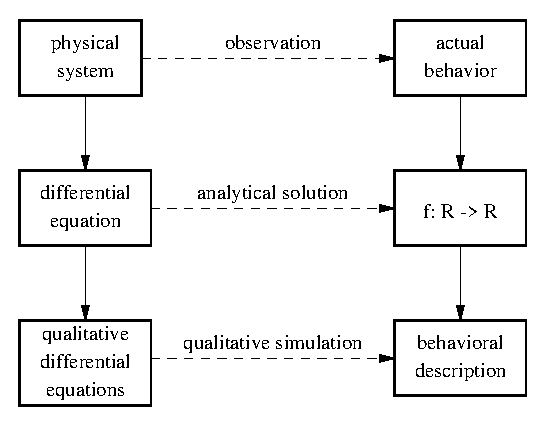
\includegraphics[width=10cm,keepaspectratio=true]{qdeode}}
%\centerline{\includegraphics[width=\the\columnwidth,keepaspectratio=true]{odeqde}}
\caption[Abstraktionsebenen eines physikalischen Sy\-stems.]
{Die verschiedenen Abstraktionsebenen eines physikalischen Sy\-stems.}
\label{fig_abstraktion}
\end{figure}

Im Gegensatz zur kontinuierlichen Simulation, welche f"ur numerische 
Eingabegr"o\3en die resultierenden Ausgabewerte berechnet, wird bei der 
qualitativen Simulation das Modell abstrakter betrachtet.
Diese abstrakte Betrachtungsweise entspricht auch eher dem menschlichen
Verst"andnis.
Gr"unde f"ur den Einsatz der qualitativen Simulation sind unter anderem:

\begin{itemize}
\item Das quantitative Wissen "uber ein System ist unvollst"andig oder 
nicht gegeben. 
\item Das Modell ist zu komplex und daher zu zeitaufwendig f"ur die 
konti\-nuier\-liche  Simulation.
\item Bestimmte Anwendungen ben"otigen gar nicht die detaillierten Ergebnisse der kontinuierlichen Simulation. Qualitative Aussagen sind ausreichend. 
\end{itemize}

Aufgrund dieser Eigenschaften wird die qualitative Simulation immer "ofter 
auch in technischen Anwendungen, wie zum Beispiel in der Proze\3- und 
Design"uberwachung oder in der Fehlerdiagnose, eingesetzt. \\

Der bekannteste Algorithmus f"ur die qualitative Simulation ist 
\QSIM~\cite{Kui94}..
Am Institut f"ur Technische Informatik wurde ein Forschungsprojekt 
gestartet, um die Laufzeit von \QSIM\ zu reduzieren. 
Im Rahmen dieses Projektes werden Coprozessoren f"ur rechenzeitintensive 
Teilfunktionen entwickelt und Parallelisierungm"oglichkeiten untersucht.


\section{Zielsetzung}

In dieser Arbeit wird die parallele Implementierung von rechenzeitintensiven 
Teil\-aufgaben von \QSIM\ aufgezeigt und bewertet.  Die Ziele der parallelen 
Implementierung werden in den folgenden Abs"atzen aufgelistet.

\begin{description}
\item{Verarbeitungszeit:}
F"ur \QSIM\ Anwendungen werden schnelle Simulatoren be\-n"otigt.
Ein Schwerpunkt des Forschungsprojektes und dieser Arbeit liegt daher darin, 
die Verarbeitungszeit gegen"uber bestehenden Implementierungen von QSIM zu 
verbessern.
\item{Skalierbarkeit:}
Ein weiterer wichtiger Aspekt einer parallelen Implementierung ist ein 
skalierbares Design.  F"ur eine h"ohere Prozessoranzahl soll auch die 
Leistung des Systems steigen.
\item{Speedup:}
Das Verh"altnis der Laufzeiten des Einprozessorsystems zum Mehrprozessorsystem 
wird untersucht und bewertet. Die Beschreibung dieses Verh"altnisses erfolgt 
mit Hilfe des Speedups.
\end{description}

Die Implementierung erfolgt auf einer Multi-DSP Architektur.  Als Prozessor 
wird der digitale Signalprozessor TMS320C40 von Texas Instruments verwendet. 
Ein Transtech Multi-C40 Board bildet die Plattform f"ur die Implementierung. 
Dieses System ist als PC-Einsteckkarte ausgef"uhrt.
Die Programmierung der Prozessoren erfolgt mit dem verteilten 
Echtzeit-Betriebssystem Virtuoso.


\section{Gliederung}

In {\bf Kapitel~2} wird \QSIM\ allgemein erl"autert. Die Ans"atze f"ur eine
parallele Implementierung werden dabei mitbehandelt.
Es zeigt sich, da\3 gewisse rechenzeitintensive Aufgaben f"ur eine parallele
Implementation geeignet sind.
Die paral\-lelisier\-baren Aufgaben werden dann charakterisiert und auf ihre 
spezifischen Eigenschaften untersucht.

In {\bf Kapitel~3} wird das Scheduling-Problem nach grundlegenden Kriterien 
kategorisiert. Mit dieser Einteilung und der Charakterisierung aus dem 
Kapitel~2 werden Schedulingverfahren beschrieben.
Es werden Heuristiken f"ur verschiedene Schedulingverfahren vorgestellt und 
die Abweichung zur Optimall"osung beschrieben. Die Heuristiken werden auch 
auf ihre Komplexit"at untersucht.

{\bf Kapitel~4} beschreibt die Implementierung und die experimentellen 
Ergebnisse.
Im ersten Abschnitt wird die Multi-DSP Architektur und das verwendete 
Betriebssystem beschrieben.
Der zweite Abschnitt be\-sch"aftigt sich mit der konkreten parallelen 
Implementierung der \QSIM\ Kernfunktionen.

Eine Diskussion der parallelen Implementierung von \QSIM\ und  einen Ausblick 
auf weitere Entwicklungen an der parallelen Implementierung von \QSIM\ werden 
in {\bf Kapitel~5} angef"uhrt und bilden den Abschlu\3 dieser Arbeit.

%Es wird empfohlen, den Text in einzelne Files aufzuteilen und diese dann
%einzubinden.  
%Beispiel: der Text ist im File Einleitung.tex und wird mit \input eigebunden.
%\input{Einleitung}

\chapter{\"{U}berschrift Kapitel zwei}
\label{kap:LabelKapitelZwei}
Neue Kapitel beginnen automatisch immer auf einer neuen Seite.

Die Schriftgr\"{o}{\ss}en f\"{u}r die \"{U}berschriften der einzelnen 
Unterabschnitte erfolgen automatisch abgestuft.  
Ab der 3.~Unterebene erfolgt keine
Numerierung mehr.

%\input{text_kapitel2}
  \section{\"{U}berschrift Abschnitt}
%  \input{text_Abschnitt21}
  \section{\"{U}berschrift n\"{a}chster Abschnitt}
%  \input{text_Abschnitt22}
  \subsection{\"{U}berschrift Unterabschnitt}
  \subsubsection{\"{U}berschrift Unter-Unterabschnitt}
  \section{\"{U}berschrift NochEinAbschnitt}
    \label{kap:WichtigerAbschnitt}
    \index{Abschnitt \ref{kap:WichtigerAbschnitt}}


\chapter{\"{U}berschrift Kapitel drei}
\label{kap:LabelKapitelDrei} Die Kapitel sollten jedenfalls die
Aufgabenstellung, den Stand der Technik, die Vorgehensweise zur
L\"{o}sung des Problems und die L\"{o}sung enthalten. Programmlistings
sollten nicht Teil der Diplomarbeit sein. Evtl. k\"{o}nnen elegante
L\"{o}sungen bzw. wesentliche Elemente dargestellt werden. Hinweise
auf den Anhang und (gek\"{u}rzte) Ausz\"{u}ge dort sind aber zul\"{a}ssig.
\section{\"{U}berschrift Abschnitt 3.1}
  %\input{text_Abschnitt31} %einzelne Files f\"{u}r Abschnitte

\begin{itemize}
\item Es sollte eine sinnvolle Aufteilung in Text-Files
(Kapitel, Abschnitte, Unterabschnitte erfolgen.
\item Ziehen Sie sinnvolle Label-Bezeichner mit den \"{U}berschriften 
mit.
\item Sortieren Sie die Bilder in Unterverzeichnisse,
gleich mit Label und Caption versehen.
\end{itemize}

\begin{enumerate}
\item Listen kann man auch numerieren.
\item Auch bei Querverweisen kann man sich auf \LaTeX\ verlassen. 
Hier wird auf Kapitel \ref{kap:LabelKapitelZwei} verwiesen.
\item Das Referenzieren funktioniert ebenfalls sehr einfach.  Setzen Sie die
Referenzen immer innerhalb eines Satzes.  Beispiel dazu sind:
\begin{itemize}
\item Wie in \cite{Voas97} gezeigt, $\ldots$ oder
\item Referenzieren von Quellen ist sehr einfach \cite{Kui94}.
\end{itemize}
Die Quellenangaben werden am besten in einer eigenen Datei erfasst 
(hier {\tt diplom.bib}) und mit dem Programm {\tt bibtex} in eine
eigene \LaTeX -Datei (hier {\tt diplom.bbl}) umgewandelt.
\end{enumerate}



\chapter{\"{U}berschrift NochEinKapitel}
   \label{kap:NochEinKapitel}

Tabellen k"onnen einfach erzeugt werden.  Ein Beispiel dazu ist
in Tabelle~\ref{tab1} angegeben.

\begin{table}[h!]
\centering
\begin{tabular}{|c|c|r|r|r|}\hline\hline
{\em observ.~variables} & {\em subspaces} & {\em sampling rate [Hz]} &
$t_{real}$ {\em [s]} & $t_{mon}$ {\em [s]}\\ \hline
           &    & 0,1 &  90,0 &  3,56  \\ \cline{3-5}
T1, T2, T3 &  1 & 1   &  90,0 &  1,26  \\ \cline{3-5}
           &    & 10  &  89,6 &  2,20  \\ \hline
           &    & 0,1 &  90,0 &110,84  \\ \cline{3-5}
T1, T2, T3 & 32 & 1   &  88,0 & 32,10  \\ \cline{3-5}
           &    & 10  &  87,7 & 26,60  \\ \hline
           &    & 0,1 & 150,0 &  4,58  \\ \cline{3-5}
T2         &  1 & 1   & 146,0 &  1,55  \\ \cline{3-5}
           &    & 10  & 145,1 &  3,33  \\ \hline
           &    & 0,1 & 150,0 &139,20  \\ \cline{3-5}
T2         & 32 & 1   & 136,0 & 29,00  \\ \cline{3-5}
           &    & 10  & 134,3 & 40,70 \\ \hline\hline
\end{tabular}
\caption[Laufzeit des Algorithmus.]
{Laufzeit des Algorithmus.  Hier kann zus"atzlicher Text angegeben werden,
der nicht im Tabellenverzeichnis aufscheint.}  
\label{tab1}
\end{table}

"Ahnliches gilt auch f"ur mathematische Formeln. Sie k"onnen entweder direkt
im Text, wie z.B.~$a^2+b^2=c^2$, oder als eigenes Element mit oder ohne
Nummerierung angegeben werden.

\begin{equation}
{\bf x}_{t} = {\bf f}({\bf x}_{t-1},{\bf u}_{t-1},{\bf p}_{t-1}) 
\label{System}
\end{equation}


\chapter{Schlu{\ss}bemerkung und Ausblick}
  \label{kap:ausblick}
  %\input{s_ausblick}

\begin{appendix}
\chapter{z.B. Begriffsbestimmung}
\section{z.B. Definitionen}
%\input{a_text}
\section{z.B. Verwendete Symbole}
%\input{a_files}
\end{appendix}

%nicht referenzierte Literaturstellen

\nocite{mseifter88,pmandl97,weiss92,weiss92a,ginthoer93}

% Literaturverzeichnis einbinden, alpha, plain, unsrt, abbrv
\newpage
%Eintrag im Inhaltsverzeichnis
\addtocounter{page}{1}
\addcontentsline{toc}{chapter}{Literaturverzeichnis}
\addtocounter{page}{-1}

\bibliographystyle{alpha}

\bibliography{diplom}

%Index File
%%\documentclass[11pt, draft, oneside]{report}
\documentclass[11pt]{report}
%\makeindex
%\usepackage{german,a4,showidx} %index an seite
\usepackage{german,a4}
%for pdfLaTeX output Bilder als .png speichern:
%\usepackage[pdftex]{graphicx} \DeclareGraphicsExtensions{.png}  \graphicspath{{bilder/png/}}
% f\"{u}r normales LaTeX->dvi, Bilder als .eps speichern:
\usepackage{graphicx} \DeclareGraphicsExtensions{.eps} \graphicspath{{bilder/eps/}}

%Definition der Seitengr"osse
\setlength{\textwidth}{15 true cm}
\setlength{\textheight}{22 true cm}
\oddsidemargin  0.5 cm
\evensidemargin 0.5 cm
\topmargin      0 cm

\selectlanguage{german}
%Beispiel fuer ein neues LaTex Kommando
\newcommand{\QSIM}{{\sc QSim}}

\begin{document}

% Die Titelseite ist immer in Deutsch (austrian), danach h\"{a}ngt es von der
% Sprache der Diplomarbeit ab. Jedenfalls muss eine Kurzfassung und
% ein Abstract existieren

%\thispagestyle{empty} 
%\selectlanguage{german}

\newpage
\vspace*{2.2 cm}
{\Large
\noindent
{\bf Kurzfassung}} \\
\vspace*{0.3 cm}

\noindent
Hier steht der deutsche Text der Kurzfassung. Eine
evtl. gek\"{u}rzte Version inklusive einiger Stichw\"{o}rter muss auch im
TUG-Online eingegeben werden.


\newpage
\selectlanguage{english}
\vspace*{2.2 cm}
{\Large
\noindent
{\bf Abstract}} \\
\vspace*{0.3 cm}

\noindent
This is the English version of the abstract.  It is also
required to submit a short English abstract including some
keywords to the TUG-Online system.

\newpage
\selectlanguage{german}
\newpage
\vspace*{2.2 cm}
{\Large
\noindent
{\bf Danksagung}} \\
\vspace*{0.3 cm}
% OPTIONAL

\noindent
Diese Diplomarbeit wurde im (Studien)Jahr am Institut f\"{u}r
Technische Informatik an der Technischen Universit\"{a}t Graz
durchgef\"{u}hrt.

\smallskip
Danksagung an alle am Institut bzw. bei Firmen, die geholfen
haben....

\medskip
Danksagung an Freunde und Freundinnen f\"{u}r das Verst\"{a}ndnis, ebenso
den Eltern und allen sonstigen Sponsoren....

\vspace{2 cm}

\noindent Graz, im Monat Jahr \hfill Name des Diplomanden

\newpage
% Inhaltsverzeichnis
\tableofcontents  

% Tabellenverzeichnis
% OPTIONAL
\listoffigures 

% Abbildungsverzeichnis
% OPTIONAL
\listoftables

%Seitennummerierung am Kopf inkl. Kapitel"uberschrift
\pagestyle{headings}
\chapter{Einleitung}
% Einleitung ist Kapitel 1
\label{kap:Einleitung} 
Dieses Dokument soll als Vorlage zum Verfassen von Diplomarbeiten am
Institut f"ur Technische Informatik der TU Graz mit Hilfe von \LaTeX\
dienen.  Es sind hier die wichtigsten Abschnitte der Diplomarbeit 
zusammengefa\3t.  Weiters werden die wichtigsten Befehle von \LaTeX\ an
einigen Beispielen kurz vorgestellt.  Dieses Vorlage erhebt keinen Anspruch
auf Vollst"andigkeit.

Die Einleitung enth\"{a}lt u.A. die Aufgabenstellung, die Vorgehensweise zur
L\"{o}sung und die Gliederung der Arbeit.  Es folgt nun ein {\bf Beispieltext}.

\section{Motivation}

Qualitative Simulation ist ein Teilbereich des {\em qualitative reasonings} 
(qualitatives Schlie\3en). Dabei wird versucht, Schlu\3folgerungen "uber 
das Verhalten von Systemen auf h"oheren Abstraktionsebenen zu ziehen.
Hauptanwendungsgebiete f"ur die qualitative Simulation sind Bereiche der 
k"unstlichen Intelligenz. 
Die Abbildung~\ref{fig_abstraktion} zeigt die verschiedenen Abstraktionsebenen eines 
Systems.  Die erste Ebene stellt das physikalische System dar. 
Durch die Beobachtung des Systems kann das Verhalten bestimmt werden.
In der zweiten Ebene wird das physikalische System mit 
Differentialgleichungen {\em (DGLen)} modelliert.  Durch eine analytischen 
Berechnung der DGLen wird eine Beschreibung des Verhaltens mit 
reell\-wertigen Funktionen erzielt.  In der kontinuierlichen Simulation 
werden h"aufig numerische Verfahren zur Berechnung dieser Funktionen 
eingesetzt.  Eine weitere Abstraktion der DGLen in qualitative DGLen 
{\em (qualitative differential equations - QDEs)} wird in der dritten Ebene 
vollzogen.  Die qualitative Simulation bestimmt aus diesem Modell eine 
qualitative Beschreibung des Systemverhaltens. 

\begin{figure} %optinale Positionsparameter [htbp]
\centerline{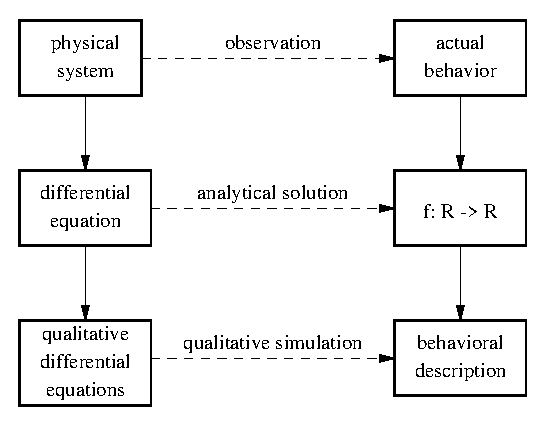
\includegraphics[width=10cm,keepaspectratio=true]{qdeode}}
%\centerline{\includegraphics[width=\the\columnwidth,keepaspectratio=true]{odeqde}}
\caption[Abstraktionsebenen eines physikalischen Sy\-stems.]
{Die verschiedenen Abstraktionsebenen eines physikalischen Sy\-stems.}
\label{fig_abstraktion}
\end{figure}

Im Gegensatz zur kontinuierlichen Simulation, welche f"ur numerische 
Eingabegr"o\3en die resultierenden Ausgabewerte berechnet, wird bei der 
qualitativen Simulation das Modell abstrakter betrachtet.
Diese abstrakte Betrachtungsweise entspricht auch eher dem menschlichen
Verst"andnis.
Gr"unde f"ur den Einsatz der qualitativen Simulation sind unter anderem:

\begin{itemize}
\item Das quantitative Wissen "uber ein System ist unvollst"andig oder 
nicht gegeben. 
\item Das Modell ist zu komplex und daher zu zeitaufwendig f"ur die 
konti\-nuier\-liche  Simulation.
\item Bestimmte Anwendungen ben"otigen gar nicht die detaillierten Ergebnisse der kontinuierlichen Simulation. Qualitative Aussagen sind ausreichend. 
\end{itemize}

Aufgrund dieser Eigenschaften wird die qualitative Simulation immer "ofter 
auch in technischen Anwendungen, wie zum Beispiel in der Proze\3- und 
Design"uberwachung oder in der Fehlerdiagnose, eingesetzt. \\

Der bekannteste Algorithmus f"ur die qualitative Simulation ist 
\QSIM~\cite{Kui94}..
Am Institut f"ur Technische Informatik wurde ein Forschungsprojekt 
gestartet, um die Laufzeit von \QSIM\ zu reduzieren. 
Im Rahmen dieses Projektes werden Coprozessoren f"ur rechenzeitintensive 
Teilfunktionen entwickelt und Parallelisierungm"oglichkeiten untersucht.


\section{Zielsetzung}

In dieser Arbeit wird die parallele Implementierung von rechenzeitintensiven 
Teil\-aufgaben von \QSIM\ aufgezeigt und bewertet.  Die Ziele der parallelen 
Implementierung werden in den folgenden Abs"atzen aufgelistet.

\begin{description}
\item{Verarbeitungszeit:}
F"ur \QSIM\ Anwendungen werden schnelle Simulatoren be\-n"otigt.
Ein Schwerpunkt des Forschungsprojektes und dieser Arbeit liegt daher darin, 
die Verarbeitungszeit gegen"uber bestehenden Implementierungen von QSIM zu 
verbessern.
\item{Skalierbarkeit:}
Ein weiterer wichtiger Aspekt einer parallelen Implementierung ist ein 
skalierbares Design.  F"ur eine h"ohere Prozessoranzahl soll auch die 
Leistung des Systems steigen.
\item{Speedup:}
Das Verh"altnis der Laufzeiten des Einprozessorsystems zum Mehrprozessorsystem 
wird untersucht und bewertet. Die Beschreibung dieses Verh"altnisses erfolgt 
mit Hilfe des Speedups.
\end{description}

Die Implementierung erfolgt auf einer Multi-DSP Architektur.  Als Prozessor 
wird der digitale Signalprozessor TMS320C40 von Texas Instruments verwendet. 
Ein Transtech Multi-C40 Board bildet die Plattform f"ur die Implementierung. 
Dieses System ist als PC-Einsteckkarte ausgef"uhrt.
Die Programmierung der Prozessoren erfolgt mit dem verteilten 
Echtzeit-Betriebssystem Virtuoso.


\section{Gliederung}

In {\bf Kapitel~2} wird \QSIM\ allgemein erl"autert. Die Ans"atze f"ur eine
parallele Implementierung werden dabei mitbehandelt.
Es zeigt sich, da\3 gewisse rechenzeitintensive Aufgaben f"ur eine parallele
Implementation geeignet sind.
Die paral\-lelisier\-baren Aufgaben werden dann charakterisiert und auf ihre 
spezifischen Eigenschaften untersucht.

In {\bf Kapitel~3} wird das Scheduling-Problem nach grundlegenden Kriterien 
kategorisiert. Mit dieser Einteilung und der Charakterisierung aus dem 
Kapitel~2 werden Schedulingverfahren beschrieben.
Es werden Heuristiken f"ur verschiedene Schedulingverfahren vorgestellt und 
die Abweichung zur Optimall"osung beschrieben. Die Heuristiken werden auch 
auf ihre Komplexit"at untersucht.

{\bf Kapitel~4} beschreibt die Implementierung und die experimentellen 
Ergebnisse.
Im ersten Abschnitt wird die Multi-DSP Architektur und das verwendete 
Betriebssystem beschrieben.
Der zweite Abschnitt be\-sch"aftigt sich mit der konkreten parallelen 
Implementierung der \QSIM\ Kernfunktionen.

Eine Diskussion der parallelen Implementierung von \QSIM\ und  einen Ausblick 
auf weitere Entwicklungen an der parallelen Implementierung von \QSIM\ werden 
in {\bf Kapitel~5} angef"uhrt und bilden den Abschlu\3 dieser Arbeit.

%Es wird empfohlen, den Text in einzelne Files aufzuteilen und diese dann
%einzubinden.  
%Beispiel: der Text ist im File Einleitung.tex und wird mit \input eigebunden.
%\input{Einleitung}

\chapter{\"{U}berschrift Kapitel zwei}
\label{kap:LabelKapitelZwei}
Neue Kapitel beginnen automatisch immer auf einer neuen Seite.

Die Schriftgr\"{o}{\ss}en f\"{u}r die \"{U}berschriften der einzelnen 
Unterabschnitte erfolgen automatisch abgestuft.  
Ab der 3.~Unterebene erfolgt keine
Numerierung mehr.

%\input{text_kapitel2}
  \section{\"{U}berschrift Abschnitt}
%  \input{text_Abschnitt21}
  \section{\"{U}berschrift n\"{a}chster Abschnitt}
%  \input{text_Abschnitt22}
  \subsection{\"{U}berschrift Unterabschnitt}
  \subsubsection{\"{U}berschrift Unter-Unterabschnitt}
  \section{\"{U}berschrift NochEinAbschnitt}
    \label{kap:WichtigerAbschnitt}
    \index{Abschnitt \ref{kap:WichtigerAbschnitt}}


\chapter{\"{U}berschrift Kapitel drei}
\label{kap:LabelKapitelDrei} Die Kapitel sollten jedenfalls die
Aufgabenstellung, den Stand der Technik, die Vorgehensweise zur
L\"{o}sung des Problems und die L\"{o}sung enthalten. Programmlistings
sollten nicht Teil der Diplomarbeit sein. Evtl. k\"{o}nnen elegante
L\"{o}sungen bzw. wesentliche Elemente dargestellt werden. Hinweise
auf den Anhang und (gek\"{u}rzte) Ausz\"{u}ge dort sind aber zul\"{a}ssig.
\section{\"{U}berschrift Abschnitt 3.1}
  %\input{text_Abschnitt31} %einzelne Files f\"{u}r Abschnitte

\begin{itemize}
\item Es sollte eine sinnvolle Aufteilung in Text-Files
(Kapitel, Abschnitte, Unterabschnitte erfolgen.
\item Ziehen Sie sinnvolle Label-Bezeichner mit den \"{U}berschriften 
mit.
\item Sortieren Sie die Bilder in Unterverzeichnisse,
gleich mit Label und Caption versehen.
\end{itemize}

\begin{enumerate}
\item Listen kann man auch numerieren.
\item Auch bei Querverweisen kann man sich auf \LaTeX\ verlassen. 
Hier wird auf Kapitel \ref{kap:LabelKapitelZwei} verwiesen.
\item Das Referenzieren funktioniert ebenfalls sehr einfach.  Setzen Sie die
Referenzen immer innerhalb eines Satzes.  Beispiel dazu sind:
\begin{itemize}
\item Wie in \cite{Voas97} gezeigt, $\ldots$ oder
\item Referenzieren von Quellen ist sehr einfach \cite{Kui94}.
\end{itemize}
Die Quellenangaben werden am besten in einer eigenen Datei erfasst 
(hier {\tt diplom.bib}) und mit dem Programm {\tt bibtex} in eine
eigene \LaTeX -Datei (hier {\tt diplom.bbl}) umgewandelt.
\end{enumerate}



\chapter{\"{U}berschrift NochEinKapitel}
   \label{kap:NochEinKapitel}

Tabellen k"onnen einfach erzeugt werden.  Ein Beispiel dazu ist
in Tabelle~\ref{tab1} angegeben.

\begin{table}[h!]
\centering
\begin{tabular}{|c|c|r|r|r|}\hline\hline
{\em observ.~variables} & {\em subspaces} & {\em sampling rate [Hz]} &
$t_{real}$ {\em [s]} & $t_{mon}$ {\em [s]}\\ \hline
           &    & 0,1 &  90,0 &  3,56  \\ \cline{3-5}
T1, T2, T3 &  1 & 1   &  90,0 &  1,26  \\ \cline{3-5}
           &    & 10  &  89,6 &  2,20  \\ \hline
           &    & 0,1 &  90,0 &110,84  \\ \cline{3-5}
T1, T2, T3 & 32 & 1   &  88,0 & 32,10  \\ \cline{3-5}
           &    & 10  &  87,7 & 26,60  \\ \hline
           &    & 0,1 & 150,0 &  4,58  \\ \cline{3-5}
T2         &  1 & 1   & 146,0 &  1,55  \\ \cline{3-5}
           &    & 10  & 145,1 &  3,33  \\ \hline
           &    & 0,1 & 150,0 &139,20  \\ \cline{3-5}
T2         & 32 & 1   & 136,0 & 29,00  \\ \cline{3-5}
           &    & 10  & 134,3 & 40,70 \\ \hline\hline
\end{tabular}
\caption[Laufzeit des Algorithmus.]
{Laufzeit des Algorithmus.  Hier kann zus"atzlicher Text angegeben werden,
der nicht im Tabellenverzeichnis aufscheint.}  
\label{tab1}
\end{table}

"Ahnliches gilt auch f"ur mathematische Formeln. Sie k"onnen entweder direkt
im Text, wie z.B.~$a^2+b^2=c^2$, oder als eigenes Element mit oder ohne
Nummerierung angegeben werden.

\begin{equation}
{\bf x}_{t} = {\bf f}({\bf x}_{t-1},{\bf u}_{t-1},{\bf p}_{t-1}) 
\label{System}
\end{equation}


\chapter{Schlu{\ss}bemerkung und Ausblick}
  \label{kap:ausblick}
  %\input{s_ausblick}

\begin{appendix}
\chapter{z.B. Begriffsbestimmung}
\section{z.B. Definitionen}
%\input{a_text}
\section{z.B. Verwendete Symbole}
%\input{a_files}
\end{appendix}

%nicht referenzierte Literaturstellen

\nocite{mseifter88,pmandl97,weiss92,weiss92a,ginthoer93}

% Literaturverzeichnis einbinden, alpha, plain, unsrt, abbrv
\newpage
%Eintrag im Inhaltsverzeichnis
\addtocounter{page}{1}
\addcontentsline{toc}{chapter}{Literaturverzeichnis}
\addtocounter{page}{-1}

\bibliographystyle{alpha}

\bibliography{diplom}

%Index File
%%\documentclass[11pt, draft, oneside]{report}
\documentclass[11pt]{report}
%\makeindex
%\usepackage{german,a4,showidx} %index an seite
\usepackage{german,a4}
%for pdfLaTeX output Bilder als .png speichern:
%\usepackage[pdftex]{graphicx} \DeclareGraphicsExtensions{.png}  \graphicspath{{bilder/png/}}
% f\"{u}r normales LaTeX->dvi, Bilder als .eps speichern:
\usepackage{graphicx} \DeclareGraphicsExtensions{.eps} \graphicspath{{bilder/eps/}}

%Definition der Seitengr"osse
\setlength{\textwidth}{15 true cm}
\setlength{\textheight}{22 true cm}
\oddsidemargin  0.5 cm
\evensidemargin 0.5 cm
\topmargin      0 cm

\selectlanguage{german}
%Beispiel fuer ein neues LaTex Kommando
\newcommand{\QSIM}{{\sc QSim}}

\begin{document}

% Die Titelseite ist immer in Deutsch (austrian), danach h\"{a}ngt es von der
% Sprache der Diplomarbeit ab. Jedenfalls muss eine Kurzfassung und
% ein Abstract existieren

%\thispagestyle{empty} 
%\selectlanguage{german}

\newpage
\vspace*{2.2 cm}
{\Large
\noindent
{\bf Kurzfassung}} \\
\vspace*{0.3 cm}

\noindent
Hier steht der deutsche Text der Kurzfassung. Eine
evtl. gek\"{u}rzte Version inklusive einiger Stichw\"{o}rter muss auch im
TUG-Online eingegeben werden.


\newpage
\selectlanguage{english}
\vspace*{2.2 cm}
{\Large
\noindent
{\bf Abstract}} \\
\vspace*{0.3 cm}

\noindent
This is the English version of the abstract.  It is also
required to submit a short English abstract including some
keywords to the TUG-Online system.

\newpage
\selectlanguage{german}
\newpage
\vspace*{2.2 cm}
{\Large
\noindent
{\bf Danksagung}} \\
\vspace*{0.3 cm}
% OPTIONAL

\noindent
Diese Diplomarbeit wurde im (Studien)Jahr am Institut f\"{u}r
Technische Informatik an der Technischen Universit\"{a}t Graz
durchgef\"{u}hrt.

\smallskip
Danksagung an alle am Institut bzw. bei Firmen, die geholfen
haben....

\medskip
Danksagung an Freunde und Freundinnen f\"{u}r das Verst\"{a}ndnis, ebenso
den Eltern und allen sonstigen Sponsoren....

\vspace{2 cm}

\noindent Graz, im Monat Jahr \hfill Name des Diplomanden

\newpage
% Inhaltsverzeichnis
\tableofcontents  

% Tabellenverzeichnis
% OPTIONAL
\listoffigures 

% Abbildungsverzeichnis
% OPTIONAL
\listoftables

%Seitennummerierung am Kopf inkl. Kapitel"uberschrift
\pagestyle{headings}
\chapter{Einleitung}
% Einleitung ist Kapitel 1
\label{kap:Einleitung} 
Dieses Dokument soll als Vorlage zum Verfassen von Diplomarbeiten am
Institut f"ur Technische Informatik der TU Graz mit Hilfe von \LaTeX\
dienen.  Es sind hier die wichtigsten Abschnitte der Diplomarbeit 
zusammengefa\3t.  Weiters werden die wichtigsten Befehle von \LaTeX\ an
einigen Beispielen kurz vorgestellt.  Dieses Vorlage erhebt keinen Anspruch
auf Vollst"andigkeit.

Die Einleitung enth\"{a}lt u.A. die Aufgabenstellung, die Vorgehensweise zur
L\"{o}sung und die Gliederung der Arbeit.  Es folgt nun ein {\bf Beispieltext}.

\section{Motivation}

Qualitative Simulation ist ein Teilbereich des {\em qualitative reasonings} 
(qualitatives Schlie\3en). Dabei wird versucht, Schlu\3folgerungen "uber 
das Verhalten von Systemen auf h"oheren Abstraktionsebenen zu ziehen.
Hauptanwendungsgebiete f"ur die qualitative Simulation sind Bereiche der 
k"unstlichen Intelligenz. 
Die Abbildung~\ref{fig_abstraktion} zeigt die verschiedenen Abstraktionsebenen eines 
Systems.  Die erste Ebene stellt das physikalische System dar. 
Durch die Beobachtung des Systems kann das Verhalten bestimmt werden.
In der zweiten Ebene wird das physikalische System mit 
Differentialgleichungen {\em (DGLen)} modelliert.  Durch eine analytischen 
Berechnung der DGLen wird eine Beschreibung des Verhaltens mit 
reell\-wertigen Funktionen erzielt.  In der kontinuierlichen Simulation 
werden h"aufig numerische Verfahren zur Berechnung dieser Funktionen 
eingesetzt.  Eine weitere Abstraktion der DGLen in qualitative DGLen 
{\em (qualitative differential equations - QDEs)} wird in der dritten Ebene 
vollzogen.  Die qualitative Simulation bestimmt aus diesem Modell eine 
qualitative Beschreibung des Systemverhaltens. 

\begin{figure} %optinale Positionsparameter [htbp]
\centerline{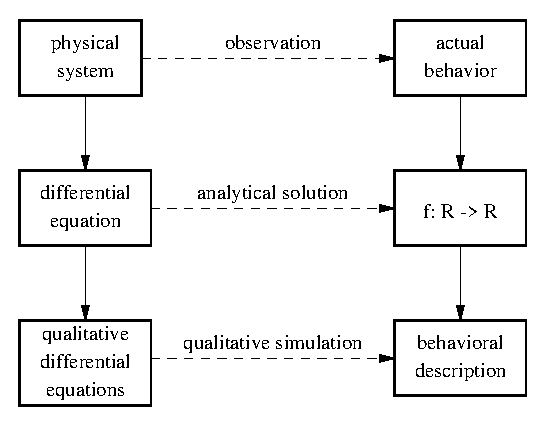
\includegraphics[width=10cm,keepaspectratio=true]{qdeode}}
%\centerline{\includegraphics[width=\the\columnwidth,keepaspectratio=true]{odeqde}}
\caption[Abstraktionsebenen eines physikalischen Sy\-stems.]
{Die verschiedenen Abstraktionsebenen eines physikalischen Sy\-stems.}
\label{fig_abstraktion}
\end{figure}

Im Gegensatz zur kontinuierlichen Simulation, welche f"ur numerische 
Eingabegr"o\3en die resultierenden Ausgabewerte berechnet, wird bei der 
qualitativen Simulation das Modell abstrakter betrachtet.
Diese abstrakte Betrachtungsweise entspricht auch eher dem menschlichen
Verst"andnis.
Gr"unde f"ur den Einsatz der qualitativen Simulation sind unter anderem:

\begin{itemize}
\item Das quantitative Wissen "uber ein System ist unvollst"andig oder 
nicht gegeben. 
\item Das Modell ist zu komplex und daher zu zeitaufwendig f"ur die 
konti\-nuier\-liche  Simulation.
\item Bestimmte Anwendungen ben"otigen gar nicht die detaillierten Ergebnisse der kontinuierlichen Simulation. Qualitative Aussagen sind ausreichend. 
\end{itemize}

Aufgrund dieser Eigenschaften wird die qualitative Simulation immer "ofter 
auch in technischen Anwendungen, wie zum Beispiel in der Proze\3- und 
Design"uberwachung oder in der Fehlerdiagnose, eingesetzt. \\

Der bekannteste Algorithmus f"ur die qualitative Simulation ist 
\QSIM~\cite{Kui94}..
Am Institut f"ur Technische Informatik wurde ein Forschungsprojekt 
gestartet, um die Laufzeit von \QSIM\ zu reduzieren. 
Im Rahmen dieses Projektes werden Coprozessoren f"ur rechenzeitintensive 
Teilfunktionen entwickelt und Parallelisierungm"oglichkeiten untersucht.


\section{Zielsetzung}

In dieser Arbeit wird die parallele Implementierung von rechenzeitintensiven 
Teil\-aufgaben von \QSIM\ aufgezeigt und bewertet.  Die Ziele der parallelen 
Implementierung werden in den folgenden Abs"atzen aufgelistet.

\begin{description}
\item{Verarbeitungszeit:}
F"ur \QSIM\ Anwendungen werden schnelle Simulatoren be\-n"otigt.
Ein Schwerpunkt des Forschungsprojektes und dieser Arbeit liegt daher darin, 
die Verarbeitungszeit gegen"uber bestehenden Implementierungen von QSIM zu 
verbessern.
\item{Skalierbarkeit:}
Ein weiterer wichtiger Aspekt einer parallelen Implementierung ist ein 
skalierbares Design.  F"ur eine h"ohere Prozessoranzahl soll auch die 
Leistung des Systems steigen.
\item{Speedup:}
Das Verh"altnis der Laufzeiten des Einprozessorsystems zum Mehrprozessorsystem 
wird untersucht und bewertet. Die Beschreibung dieses Verh"altnisses erfolgt 
mit Hilfe des Speedups.
\end{description}

Die Implementierung erfolgt auf einer Multi-DSP Architektur.  Als Prozessor 
wird der digitale Signalprozessor TMS320C40 von Texas Instruments verwendet. 
Ein Transtech Multi-C40 Board bildet die Plattform f"ur die Implementierung. 
Dieses System ist als PC-Einsteckkarte ausgef"uhrt.
Die Programmierung der Prozessoren erfolgt mit dem verteilten 
Echtzeit-Betriebssystem Virtuoso.


\section{Gliederung}

In {\bf Kapitel~2} wird \QSIM\ allgemein erl"autert. Die Ans"atze f"ur eine
parallele Implementierung werden dabei mitbehandelt.
Es zeigt sich, da\3 gewisse rechenzeitintensive Aufgaben f"ur eine parallele
Implementation geeignet sind.
Die paral\-lelisier\-baren Aufgaben werden dann charakterisiert und auf ihre 
spezifischen Eigenschaften untersucht.

In {\bf Kapitel~3} wird das Scheduling-Problem nach grundlegenden Kriterien 
kategorisiert. Mit dieser Einteilung und der Charakterisierung aus dem 
Kapitel~2 werden Schedulingverfahren beschrieben.
Es werden Heuristiken f"ur verschiedene Schedulingverfahren vorgestellt und 
die Abweichung zur Optimall"osung beschrieben. Die Heuristiken werden auch 
auf ihre Komplexit"at untersucht.

{\bf Kapitel~4} beschreibt die Implementierung und die experimentellen 
Ergebnisse.
Im ersten Abschnitt wird die Multi-DSP Architektur und das verwendete 
Betriebssystem beschrieben.
Der zweite Abschnitt be\-sch"aftigt sich mit der konkreten parallelen 
Implementierung der \QSIM\ Kernfunktionen.

Eine Diskussion der parallelen Implementierung von \QSIM\ und  einen Ausblick 
auf weitere Entwicklungen an der parallelen Implementierung von \QSIM\ werden 
in {\bf Kapitel~5} angef"uhrt und bilden den Abschlu\3 dieser Arbeit.

%Es wird empfohlen, den Text in einzelne Files aufzuteilen und diese dann
%einzubinden.  
%Beispiel: der Text ist im File Einleitung.tex und wird mit \input eigebunden.
%\input{Einleitung}

\chapter{\"{U}berschrift Kapitel zwei}
\label{kap:LabelKapitelZwei}
Neue Kapitel beginnen automatisch immer auf einer neuen Seite.

Die Schriftgr\"{o}{\ss}en f\"{u}r die \"{U}berschriften der einzelnen 
Unterabschnitte erfolgen automatisch abgestuft.  
Ab der 3.~Unterebene erfolgt keine
Numerierung mehr.

%\input{text_kapitel2}
  \section{\"{U}berschrift Abschnitt}
%  \input{text_Abschnitt21}
  \section{\"{U}berschrift n\"{a}chster Abschnitt}
%  \input{text_Abschnitt22}
  \subsection{\"{U}berschrift Unterabschnitt}
  \subsubsection{\"{U}berschrift Unter-Unterabschnitt}
  \section{\"{U}berschrift NochEinAbschnitt}
    \label{kap:WichtigerAbschnitt}
    \index{Abschnitt \ref{kap:WichtigerAbschnitt}}


\chapter{\"{U}berschrift Kapitel drei}
\label{kap:LabelKapitelDrei} Die Kapitel sollten jedenfalls die
Aufgabenstellung, den Stand der Technik, die Vorgehensweise zur
L\"{o}sung des Problems und die L\"{o}sung enthalten. Programmlistings
sollten nicht Teil der Diplomarbeit sein. Evtl. k\"{o}nnen elegante
L\"{o}sungen bzw. wesentliche Elemente dargestellt werden. Hinweise
auf den Anhang und (gek\"{u}rzte) Ausz\"{u}ge dort sind aber zul\"{a}ssig.
\section{\"{U}berschrift Abschnitt 3.1}
  %\input{text_Abschnitt31} %einzelne Files f\"{u}r Abschnitte

\begin{itemize}
\item Es sollte eine sinnvolle Aufteilung in Text-Files
(Kapitel, Abschnitte, Unterabschnitte erfolgen.
\item Ziehen Sie sinnvolle Label-Bezeichner mit den \"{U}berschriften 
mit.
\item Sortieren Sie die Bilder in Unterverzeichnisse,
gleich mit Label und Caption versehen.
\end{itemize}

\begin{enumerate}
\item Listen kann man auch numerieren.
\item Auch bei Querverweisen kann man sich auf \LaTeX\ verlassen. 
Hier wird auf Kapitel \ref{kap:LabelKapitelZwei} verwiesen.
\item Das Referenzieren funktioniert ebenfalls sehr einfach.  Setzen Sie die
Referenzen immer innerhalb eines Satzes.  Beispiel dazu sind:
\begin{itemize}
\item Wie in \cite{Voas97} gezeigt, $\ldots$ oder
\item Referenzieren von Quellen ist sehr einfach \cite{Kui94}.
\end{itemize}
Die Quellenangaben werden am besten in einer eigenen Datei erfasst 
(hier {\tt diplom.bib}) und mit dem Programm {\tt bibtex} in eine
eigene \LaTeX -Datei (hier {\tt diplom.bbl}) umgewandelt.
\end{enumerate}



\chapter{\"{U}berschrift NochEinKapitel}
   \label{kap:NochEinKapitel}

Tabellen k"onnen einfach erzeugt werden.  Ein Beispiel dazu ist
in Tabelle~\ref{tab1} angegeben.

\begin{table}[h!]
\centering
\begin{tabular}{|c|c|r|r|r|}\hline\hline
{\em observ.~variables} & {\em subspaces} & {\em sampling rate [Hz]} &
$t_{real}$ {\em [s]} & $t_{mon}$ {\em [s]}\\ \hline
           &    & 0,1 &  90,0 &  3,56  \\ \cline{3-5}
T1, T2, T3 &  1 & 1   &  90,0 &  1,26  \\ \cline{3-5}
           &    & 10  &  89,6 &  2,20  \\ \hline
           &    & 0,1 &  90,0 &110,84  \\ \cline{3-5}
T1, T2, T3 & 32 & 1   &  88,0 & 32,10  \\ \cline{3-5}
           &    & 10  &  87,7 & 26,60  \\ \hline
           &    & 0,1 & 150,0 &  4,58  \\ \cline{3-5}
T2         &  1 & 1   & 146,0 &  1,55  \\ \cline{3-5}
           &    & 10  & 145,1 &  3,33  \\ \hline
           &    & 0,1 & 150,0 &139,20  \\ \cline{3-5}
T2         & 32 & 1   & 136,0 & 29,00  \\ \cline{3-5}
           &    & 10  & 134,3 & 40,70 \\ \hline\hline
\end{tabular}
\caption[Laufzeit des Algorithmus.]
{Laufzeit des Algorithmus.  Hier kann zus"atzlicher Text angegeben werden,
der nicht im Tabellenverzeichnis aufscheint.}  
\label{tab1}
\end{table}

"Ahnliches gilt auch f"ur mathematische Formeln. Sie k"onnen entweder direkt
im Text, wie z.B.~$a^2+b^2=c^2$, oder als eigenes Element mit oder ohne
Nummerierung angegeben werden.

\begin{equation}
{\bf x}_{t} = {\bf f}({\bf x}_{t-1},{\bf u}_{t-1},{\bf p}_{t-1}) 
\label{System}
\end{equation}


\chapter{Schlu{\ss}bemerkung und Ausblick}
  \label{kap:ausblick}
  %\input{s_ausblick}

\begin{appendix}
\chapter{z.B. Begriffsbestimmung}
\section{z.B. Definitionen}
%\input{a_text}
\section{z.B. Verwendete Symbole}
%\input{a_files}
\end{appendix}

%nicht referenzierte Literaturstellen

\nocite{mseifter88,pmandl97,weiss92,weiss92a,ginthoer93}

% Literaturverzeichnis einbinden, alpha, plain, unsrt, abbrv
\newpage
%Eintrag im Inhaltsverzeichnis
\addtocounter{page}{1}
\addcontentsline{toc}{chapter}{Literaturverzeichnis}
\addtocounter{page}{-1}

\bibliographystyle{alpha}

\bibliography{diplom}

%Index File
%\input{diplom.ind}

\end{document}


\end{document}


\end{document}


\end{document}
